% Part 2 chapter carrying "Dark Energy or Sector Tension? IAM Confrontation with DESI Full-Shape Growth Rates and Joint Weak Lensing" (
% Mar 2026) in its order. Read in full 2026-10-02 (934 lines, 50-line ledger). Numbers: docs/verification/scripts/verify_sector_tension.py;
% two-ruler mock: docs/verification/observations/TWO_RULER_DESI_TEST.md. Check: observations/SECTOR_TENSION_CHECK.md. Naming rule applied.
\chapter{Dark energy or two rulers?}\label{ch:sectortension}

\section*{The place}
The cosmic horizon (Chapter~\ref{ch:surfaces}). Matter writes the record and feels $\mu<1$; light writes nothing and keeps $\Sigma=1$. Any analysis that
puts observables from the two sectors into one fluid fit can read the difference as something else. This chapter asks whether DESI's evidence for
evolving dark energy is that.

\section{The observation}
\observed\ DESI DR2 BAO with the CMB and supernovae prefers $w_0>-1$, $w_a<0$~\cite{DESI2025}:
\begin{center}\small\begin{tabular}{lccc}\toprule
Data & $w_0$ & $w_a$ & $z$ where $w=-1$\\\midrule
DESI + CMB & $-0.42\pm0.21$ & $-1.75\pm0.58$ & 0.50\\
DESI + CMB + Pantheon+~\cite{Brout2022} & $-0.838\pm0.055$ & $-0.62^{+0.22}_{-0.19}$ & 0.35\\
DESI + CMB + Union3~\cite{Rubin2025} & $-0.667\pm0.088$ & $-1.09^{+0.31}_{-0.27}$ & 0.44\\
DESI + CMB + DES Y5~\cite{DESY5SN2024} & $-0.752\pm0.057$ & $-0.86^{+0.23}_{-0.20}$ & 0.41\\\bottomrule
\end{tabular}\end{center}
at $3.1$, $2.8$, $3.8$ and $4.2\sigma$. Analyses of the internal consistency of these fits (MNRAS Lett.\ 542, L24; arXiv:2504.04417) argue that the
preference may come from tension between data sets rather than from the dark energy itself, without naming a mechanism.

\section{The sector assignment}
\begin{itemize}
\item \emph{Photon ruler} ($\Lambda$CDM): the CMB acoustic angle, BAO angles $D_M/r_d$ and $D_H/r_d$, and the lensing relation between potential
and density ($\Sigma=1$).
\item \emph{Matter ruler}: growth ($f\sigma_8$, peculiar velocities), the dynamical response of matter ($\mu<1$), and the expansion rate measured by
matter, $H_m^2=H^2+\beta_mE(a)H_0^2$, giving $H_0^{\rm m}=67.16\sqrt{1+\beta_m}=72.26$ against the photon $67.16$. \calc
\item \emph{Supernovae} are standard candles in galaxies, on timelike worldlines: the matter ruler. Their distances are read with light, and with
the magnitude free the supernova fit is exactly flat in $H_0$ (Chapter~\ref{ch:dsvalidation}).
\end{itemize}

\section{Growth at the DESI redshifts}

\begin{figure}[htbp]\centering
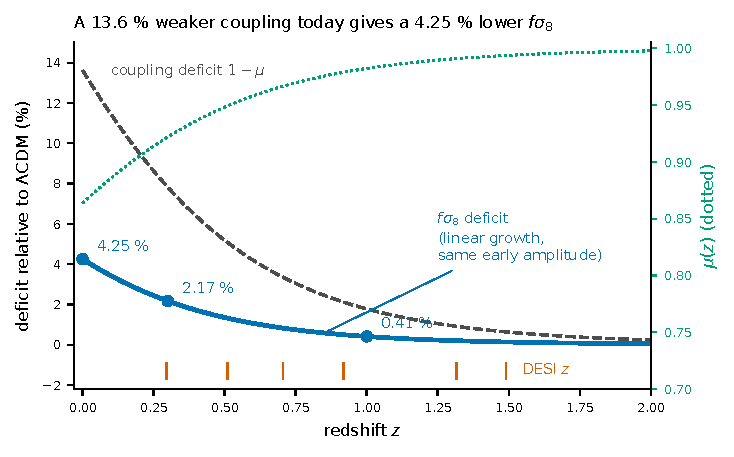
\includegraphics[width=0.8\textwidth]{figures/part2/fig_mu_fsigma8.pdf}
\caption{The coupling and the growth it produces, on one panel. Dotted (right axis): $\mu(z)=H^2/(H^2+\beta_mE(a)H_0^2)$. Dashed: the coupling deficit $1-\mu$, 13.6\,\% today, which is not a growth deficit. Solid: the deficit of $f\sigma_8$ against $\Lambda$CDM from the linear growth equation with the same early amplitude, 4.25\,\% at $z=0$, 2.17\,\% at $z=0.3$ and 0.41\,\% at $z=1$. Ticks: the DESI DR1 tracer redshifts (BGS, LRG1--3, ELG2, QSO), where the full-shape errors are 8--13\,\% per bin. Planck 2018 background ($\Omega_m=0.3153$), $\beta_m=0.15765$; \texttt{docs/verification/scripts/\allowbreak{}verify\_sector\_tension.py}. \calc}\label{fig:mu_fsigma8}
\end{figure}
The coupling deficit $1-\mu$ is not the growth deficit. With the same early amplitude, the exact coupling gives: \calc
\begin{center}\small\begin{tabular}{lcccc}\toprule
Tracer & $z$ & $1-\mu$ & $f\sigma_8$ deficit & $E_G$ change\\\midrule
BGS & 0.295 & 7.9\,\% & 2.2\,\% & $+1.9\,\%$\\ LRG1 & 0.510 & 5.1\,\% & 1.3\,\% & $+1.1\,\%$\\ LRG2 & 0.706 & 3.3\,\% & 0.8\,\% & $+0.7\,\%$\\
LRG3 & 0.919 & 2.1\,\% & 0.5\,\% & $+0.4\,\%$\\ ELG2 & 1.317 & 0.9\,\% & 0.2\,\% & $+0.2\,\%$\\ QSO & 1.491 & 0.6\,\% & 0.1\,\% & $+0.1\,\%$\\
today & 0 & 13.6\,\% & 4.25\,\% & $+3.6\,\%$\\\bottomrule
\end{tabular}\end{center}
DESI DR1 full-shape $f\sigma_8$ errors~\cite{DESI2024V} are $8$--$13\,\%$ per bin, so the data cannot yet separate the two: on the six DESI bins $\chi^2$ is
$4.51$ ($\Lambda$CDM) and $5.24$ (informational term, MGCAMB form), and on SDSS DR16~\cite{Alam2021} $6.19$ and $6.95$. \calc\ The statistic $E_G=\Omega_{m0}\Sigma/f$
is the cleanest single signature: $\Sigma=1$ with a lower $f$ raises it, by $1.8\,\%$ at $z=0.3$. \calc

\section{The clustering amplitude}
The Level 2 chains give $\sigma_8=0.7998\pm0.0058$ against $0.8087\pm0.0059$, so $S_8=0.822\pm0.011$ against $0.830$. \fitted The joint analysis of
KiDS-Legacy and DES Y3 cosmic shear with DESI DR1 BAO and Pantheon+ gives $\sigma_8=0.802^{+0.022}_{-0.018}$~\cite{Stolzner2025}, $0.1\sigma$ from the
chain value. \observed{} On $S_8$ the lensing surveys now disagree with each other: KiDS-Legacy cosmic shear gives $0.815^{+0.016}_{-0.021}$~\cite{Wright2025},
$0.4\sigma$ below the IAM value; DES Y3 galaxy clustering with weak lensing gives $0.776\pm0.017$~\cite{DESY3} ($2.3\sigma$ below) and HSC Y3 cosmic shear
$0.776^{+0.032}_{-0.033}$~\cite{HSCY3Dalal} ($1.4\sigma$ below). \observed\ (values) \calc\ (offsets, with the error on the side facing $0.822$ added in quadrature to $\pm0.011$) The IAM shift is in the direction of the lower values and
does not close the gap to them (Chapter~\ref{ch:s8trend}). With $\Sigma=1$ the lensing amplitude follows $\delta_m$: CMB lensing power is lower by $0.08\,\%$,
below any current measurement.

\section{The phantom crossing}

\begin{figure}[htbp]\centering
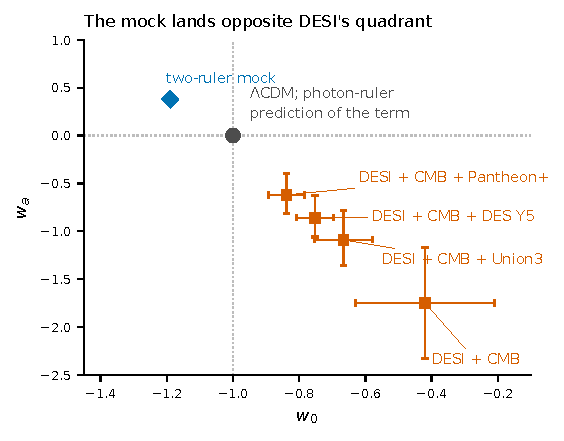
\includegraphics[width=0.62\textwidth]{figures/part2/fig_w0wa.pdf}
\caption{DESI DR2 $w_0$--$w_a$ fits with the CMB and with each supernova sample ~\cite{DESI2025} \observed, against $\Lambda$CDM, which is the informational term's prediction for photon-ruler distances, and the two-ruler mock (DESI DR2 BAO and the CMB on the photon ruler, 1,550 supernovae on $H_m$, magnitude free; $w_0=-1.19$, $w_a=+0.38$) \calc, which lands in the opposite quadrant.}\label{fig:w0wa}
\end{figure}
The sector-tension reading is that a one-fluid fit to $\Lambda$CDM distances and weaker growth must invent $w(z)\neq-1$. Three facts decide it.
\begin{enumerate}
\item The DR2 $w_0w_a$ fits use distances only --- BAO, the CMB and supernovae. No growth data enter them, so mixing distances with growth cannot be
what moves them. \observed
\item Supernovae on the matter ruler with the shape $H_m(z)$ do mix two rulers in a distance-only fit. The mock (DESI DR2 BAO and the CMB on the
photon ruler, 1,550 supernovae on $H_m$, magnitude free) gives $w_0=-1.19$, $w_a=+0.38$: the opposite quadrant to DESI. \calc
\item The real supernova data reject that shape. On Pantheon+ with full covariance~\cite{Brout2022}, applying $H_m$ to the supernova distances costs
$\Delta\chi^2=+23.6$; the supernova geometry is $\Lambda$CDM, and the matter ruler enters only through the calibration, which the free magnitude absorbs. \calc
\end{enumerate}
So the informational term predicts photon-ruler distances that are $\Lambda$CDM, $w=-1$, and it does not produce DESI's preference. If that preference
holds, it is not this term. \prediction

\section{Signatures}
$\mu$ depends on time only, so the growth change is scale independent. $\Sigma=1$, so lensing follows $\delta_m$ and $E_G$ rises. The values are
$\mu_0=-0.136$ and $\Sigma_0=0$. \prediction\ The Level~1 free-$\mu_0$ chain with redshift-space distortions reaches the upper prior edge; its
median is $+0.064$ and its one-sided 90\,\% lower bound $-0.204$, so the prediction lies inside the interval, and so does general relativity
(Chapter~\ref{ch:latetime}). \fitted\ Euclid's published forecasts bracket the test of the IAM $\mu(z)$ from about $0.3\sigma$ (conservative scale cuts) to about $7\sigma$ (smallest
scales modelled), and a forecast made with the IAM $\mu(z)$ itself is still to be done (Chapter~\ref{ch:latetime}). The survey timeline is in Chapter~\ref{ch:surveys}.

\section{Status}
The sector assignment and the growth and lensing signatures are predictions of the informational term, with $\mu_0=-0.136$ \prediction; the $H_0$
split, $67.16$ and $72.26$, follows from the Level~2 chains \calc. Calculated here: the growth deficits at the DESI redshifts are $0.1$--$2.2\,\%$,
below current errors, and the DESI phantom crossing is not produced by the informational term. \calc
